% general motivation - we are thinking to use cold atoms, quantum computing 
% spin liquids, etc to motivate the fact that there is enough data floating 
% around to use AI to do something. 
Breakthroughs in cold atom experiments, advances in quantum computing,
developments in spin liquids, and the proliferating importance of quantum
critical phenomena, in the shadow of the rapidly growing field of artificial
intelligence compel the application of machine learning techniques to difficult
quantum problems.  The exponential complexity inherent to solving quantum
problems dictates data should be used judiciously rather than be discarded. In an age
where data can drive unparalleled discoveries,
extremely-expensive-to-aquire data such as measurements of the D-wave machine
or Bloch's cold atom chains can be used by the community to distill new
information.  

% context - historical and otherwise, to lay out the problem 

% how the approach improved upon existing or solves a problem in the literature 
Here we have pioneered a method to predict quantum critical phenomena
using machine learning in the absence of direct exposure to states on either
side of the transition.  

% results and implication 
Although we only apply this to spin models, the general nature of the problem cannot 
be understated. We have developed 

\begin{figure}
	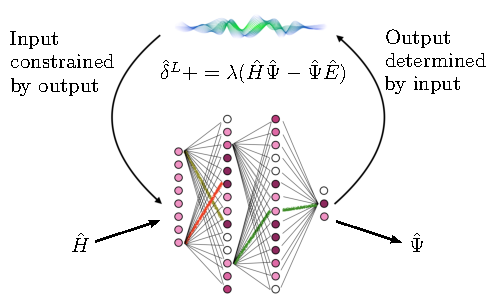
\includegraphics{figures/schematic}
	\caption{Cartoon demonstrating the self-consistency between the inputs and 
	outputs via the Schr\"{o}dinger equation.}
	\label{schematic}
\end{figure}

% other idea.... can we use the D-wave machine to generate quantum states randomly, then 
% combine with the ED method of 2D Ising model to really learn something?
